
%% main file


\documentclass[a4paper,11pt,english]{report} %book, report, article
\usepackage[english]{babel} %%%para separar correctamente las palabras de multitud de idiomas%%%
\usepackage[utf8]{inputenc} %%%Este paquete permite poner acentos directamente%%%

\usepackage{indentfirst} %%%Indentado de primera línea de cada párrafo%%%
\usepackage{parskip} %%% add some vspace between paragraphs
\setlength{\parindent}{15pt}

\usepackage[gen]{eurosym} %soporte para el comando \euro
\usepackage{mathtools}
\usepackage{amssymb}
\usepackage{graphicx} % Required for including pictures
%\usepackage{epstopdf} %para poder usar imagenes eps%
%\DeclareGraphicsExtensions{.pdf,.jpeg,.jpg,.png,.eps}
\usepackage{float} % Allows putting an [H] in \begin{figure} to specify the exact location of the figure

\usepackage[bindingoffset=0.5cm]{geometry}
%\usepackage[Sonny]{fncychap}
\usepackage[Lenny]{fncychap}
\usepackage[T1]{fontenc}
\usepackage{palatino}
\usepackage{tabularx}
\usepackage{multirow}

\usepackage[colorlinks=true, linkcolor=blue, filecolor=black, citecolor=black, urlcolor=blue]{hyperref}

\usepackage{changepage} % For the adjustwidth environment in 2ndpage
\usepackage{listings}
\usepackage{color}
\usepackage{gensymb}

\usepackage{fancyhdr}

%% Shortcut command for referencing floats
\newcommand{\figref}[1]{Figure~\ref{fig:#1}}
\newcommand{\figsref}[2]{Figures~\ref{fig:#1}~and~\ref{fig:#2}}
\newcommand{\figtoref}[2]{Figures~\ref{fig:#1}~through~\ref{fig:#2}}

\newcommand{\tblref}[1]{Table~\ref{tbl:#1}}
\newcommand{\eref}[1]{Equation~\ref{eq:#1}}
\newcommand{\esref}[2]{Equations~\ref{eq:#1}~and~\ref{eq:#2}}
\newcommand{\etoref}[2]{Equations~\ref{eq:#1}~through~\ref{eqn:#2}}

\newcommand{\secref}[1]{Section~\ref{sec:#1}}
\newcommand{\subsecref}[1]{Section~\ref{subsec:#1}}
\newcommand{\subsubsecref}[1]{Section~\ref{subsubsec:#1}}
\newcommand{\charef}[1]{Chapter~\ref{chapter:#1}}
\newcommand{\aref}[1]{Appendix~\ref{apndx:#1}}

\newcommand{\etal}{\mbox{\emph{et al. }}}
\newcommand{\etals}{\mbox{\emph{et al.}'s }}
\newcommand{\ie}{\mbox{\emph{i.e.\\}}}
\newcommand{\eg}{\mbox{\emph{e.g.\\}}}
\newcommand{\ignore}[1]{}


\hyphenation{exam-ple}          %And not exa-mple
\hyphenation{WBSNs}
\hyphenation{des-cribed}
\hyphenation{know-ledge}
\hyphenation{Never-theless}

%% INICIO DOCUMENTO
\begin{document}

\pagestyle{empty}

%*******************************************************
% Titlepage
%*******************************************************



\begin{titlepage}
\setlength{\headheight}{0pt}
\setlength{\footskip}{0pt}
\setlength{\topmargin}{0pt}

\begin{adjustwidth}{-1cm}{-3cm}
\begin{center}
\LARGE
\textsc{Universidad Politécnica de Madrid}

	\smallskip

    \hfill
	\\
	\textsc{Escuela Técnica Superior\\ de Ingenieros de Telecomunicación}\\ 


        
\includegraphics[width=8cm]{images/etsit}


	\textsc{\textbf{Trabajo Fin de Máster}}\\

    \smallskip
    \textsc{\textbf{Máster Universitario en Ingeniería Biomédica}}\\
	
    \bigskip
	\hfill
    \\
    
    \textsc{Algorithms for Real-Time \\ Symptomatic Crisis Prediction in Migraine} \\ %\bigskip

	\bigskip
    \hfill
    \\

	\textsc{María Irene de Orbe Izquierdo}
	\vspace{0.5cm}
    \hfill
    \\
	\textsc{2015}
        


        %\mySubtitle \\ \medskip   
        %\myDegree \\
        %\myDepartment \\                            
        %\myFaculty \\
        %\myUni \\ \bigskip

        %\myTime

        %\vfill                      

    \end{center}  
  \end{adjustwidth}       
\end{titlepage}   
\thispagestyle{empty}


\cleardoublepage
%*******************************************************
% Titlepage
%*******************************************************
\begin{titlepage}
\setlength{\headheight}{0pt}
\setlength{\footskip}{0pt}
\setlength{\topmargin}{0pt}

\begin{center}

\begin{figure}[ht]
\begin{minipage}[b]{0.45\linewidth}
\centering
\vfill  

\includegraphics[width=6cm]{images/etsit_small}
\end{minipage}
\hspace{2cm}
\begin{minipage}[b]{0.45\linewidth}
\centering
\vfill  

\includegraphics[width=6cm]{images/gbt}
\end{minipage}
\end{figure}


\vspace*{1cm}

\LARGE
\textsc{Universidad Politécnica de Madrid}

\smallskip
\hfill
\\
\textsc{Escuela Técnica Superior\\ de Ingenieros de Telecomunicación}\\ 
\smallskip
\hfill
\\
Departamento de Tecnología Fotónica\\
Grupo de Bioingeniería y Telemedicina\\

\vspace*{2cm} 
\textsc{\textbf{Trabajo Fin de Máster}}\\
{\Large \textsc{\textbf{Máster Universitario en Ingeniería Biomédica}}}\\

\vspace*{2cm} 
\textsc{Algorithms for Real-Time \\ Symptomatic Crisis Prediction in Migraine} \\ %\bigskip

\vspace*{1cm} 
\textsc{María Irene de Orbe Izquierdo}
\vspace{0.5cm}
\hfill
\\
\textsc{2015}
        


        %\mySubtitle \\ \medskip   
        %\myDegree \\
        %\myDepartment \\                            
        %\myFaculty \\
        %\myUni \\ \bigskip

        %\myTime

        %\vfill                      

    \end{center}      
\end{titlepage}   
\thispagestyle{empty}


\cleardoublepage
%\newlength{\vertspace}
%\setlength{\vertspace}{5pt}
%\begin{titlepage}



\begin{center}
\large
\textsc{\textbf{Trabajo Fin de Máster}}\\
\end{center}

\vspace*{3cm}

\begin{tabular}{p{3cm}l}
Título:&Algorithms for Real-Time Symptomatic\\
&Crisis Prediction in Migraine\\
\end{tabular}


\vspace*{0.5cm}

\begin{tabular}{p{3cm}l}
Autor:&D\textsuperscript{a}. María Irene de Orbe Izquierdo\\
Tutor:&D. José Luis Ayala Rodrigo\\
Ponente:&D\textsuperscript{a}. María Elena Hernando Pérez\\
\end{tabular}

\vspace*{2.5cm}
Tribunal:

\vspace*{0.5cm}
\begin{tabular}{p{3cm}l}
%	\underline{Committee Member} && \hfill Signature and Date\\[\vertspace]
	Presidente:&D. Enrique Javier Gómez Aguilera\\
	Vocal:&D\textsuperscript{a}. Álvaro Guitérrez Martín\\
	Secretario:&D\textsuperscript{a}. María Elena Hernando Pérez\\
\end{tabular}


\vspace*{1.5cm}


Calificación:

\vspace*{2cm}

\begin{flushright}
Madrid, a \ \ \ \  de julio de 2015
\end{flushright}

%\end{titlepage}
\thispagestyle{empty}

\cleardoublepage


\chapter*{}
\thispagestyle{empty}

\begingroup
\begin{flushleft}
\itshape
agradecimientos\\
bla\\
bla...
\end{flushleft}
\endgroup

\cleardoublepage

%% ESTRUCTURA DEL DOCUMENTO
\chapter*{}
\subsection*{Summary}
%\chapter*{} 
%\subsection*{Summary}

\thispagestyle{empty} 
 








\vspace*{0.5cm} 


\subsubsection*{Key  words:} real biometric  signals, algorithms, artificial neural networks, migraine, prediction 
 
\clearpage 
\thispagestyle{empty}


\subsection*{Resumen}

%\subsection*{Resumen}
\thispagestyle{empty}  

La migraña es una enfermedad frecuente que se caracteriza por recurrentes dolores de cabeza. Se trata de una patología paralizante en cuanto a que afecta a la vida personal, familiar, laboral y social de la persona que la sufre. Además, su tratamiento médico supone un alto porcentaje en los costes totales de los sistemas sanitarios.

Aunque existen síntomas característicos que preceden a la migraña, éstos no suelen manifestarse con suficiente anticipación como para que las medicinas sean efectivas y neutralicen el dolor. No obstante, dado que los pacientes son capaces de reconocer dichos síntomas, creemos que debe existir una base intrínseca, fisiológica y medible que pueda ser detectada con suficiente antelación para resolver el problema de los medicamentos.

Con el objetivo de medir estas condiciones subyacentes y ser capaces de predecir el dolor de cabeza, en este proyecto proponemos, diseñamos y evaluamos algunos métodos de \emph{data mining} basados en Redes Neuronales Artificiales.

Las señales de entras de las redes analizadas son variabels fisiológicas que fueron monitorizadas previamente de pacientes reales. La señal objetivo de cada episodio migrañoso fue construida a partir de la curva de evolución de los síntomas y el dolor registrada manualmente por el paciente. Por lo tanto, el trabajo llevado a cabo comprende también el proceso de adaptación de las señales monitorizadas para que puedas ser utilizadas con las redes neuronales desarrolladas.

Entre las diferentes topologías estudiadas, empezamos implementando el más simple perceptrón y acabamos analizando las novedosas redes neuronales pulsantes. Entremedias, evaluamos dos tipos de redes dinámicas: las \emph{Time Delay} y, entre las recurrentes, las que implementan el modelo NARX. Estudiamos también cómo los diferentes valores de los parámetros que define cada topología afecta a la salida de la red y, por consiguiente, a la predicción.

Mientras que el Perceptrón parece no adaptarse a nuestro objetivo por su falta de memoria, las redes dinámicas arrojaron mejores resultados. Más concretamente, con el modelo NARX conseguimos predecir migrañas con horizontes de predicción entorno al centenar de minutos.
Los resultados obtenidos con las redes pulsantes, las cuales incorporan específicamente información espacio-temporal, no fueron tan positivos como se esperaban. No obstante, han dado la impresión de tener un enorme potencial en nuestro escenario, por lo que más experimentos deberían hacerse en un futuro con este tipo de redes neuronales artificales.

A la vista de lo dicho anteriormente sobre el modelo NARX, la predicción de migraña a partir de sus síntomas puede ser ya una realidad. Esto significa que el 6\% de las mujeres y el 8\% de los hombres del mundo que la sufren podrán tomarse sus medicinas con suficiente tiempo de antelación como para que la actuación del tratamiento sea completa y eficaz, con el consecuente incremento de la satisfacción del paciente y la reducción de los costes sanitarios.




\vspace*{0.5cm} 
 
\subsubsection*{Palabras  clave:}  señales biométricas reales, algoritmos, redes neuronales artificiales, migraña, predicción



\pagestyle{plain}
\pagenumbering{roman}

\tableofcontents
\listoffigures
\listoftables
% This line needed to avoid \listoftables starting with page 1 (roman!)
\cleardoublepage

\pagestyle{empty}
\chapter*{Glossary}
%\chapter*{Glossary} 
 
\begin{itemize} 

\item[\textbf{ANN}] Artificial Neural Network
\item[\textbf{ANS}] Autonomic Nervous System
\item[\textbf{ECG}] ElectroCardioGram
\item[\textbf{EDA}] ElectroDermal Activity
\item[\textbf{HR}] Heart Rate
\item[\textbf{NARX}] Nonlinear AutoRegressive with eXogenous input
\item[\textbf{PPG}] PhotoPlesthymoGram
\item[\textbf{SNN}] Spiking Neural Network
\item[\textbf{SpO2}] 
\item[\textbf{TDNN}] Time Delay Neural Network
\item[\textbf{WBSN}] Wireless Body Sensor Network

\end{itemize} 


\cleardoublepage

\pagenumbering{arabic}
\pagestyle{headings}

%The first page of every chapter gets the plain page style internally; you can change this behaviour by redefining the plain style:
\fancypagestyle{plain}{%
	\fancyhf{} % clear all header and footer fields
	\renewcommand{\headrulewidth}{0pt}
	\renewcommand{\footrulewidth}{0pt}
	}


\chapter{Introduction}
%\chapter{Introduction} 
\label{chapter:introduction}

The ageing population in Europe, not healthy lifestyles and the increase of chronic diseases are resulting in a general demand increment of health attention and resources \cite{pmid18843167}. This context and the fast development of information and communication technologies (ICT) give space for the e-Health concept: the ICT application to health field.

Among e-Health components are the electronic clinical history, telemedicine, e-Learning,  continuous education in ICT, standardization and interoperability and the mobile health (m-Health) \cite{OPSOMSEstrategia}. The last mentioned component, gives name to the medicine supported by mobile devices such as tablets and smartphones, monitoring artifacts, PDAs and other wireless gadgets \cite{kay2011mhealth}. The group interaction constitutes the named Wireless Body Sensor Networks (WBSN), a booming technology due to its wide application to the telemedicine and monitoring field. m-Health belongs to a wider stage, where a mass WBSN deployment supposes two aspects to take into account: the first one, the data generation susceptible of processing in data centers; the latter, the necessity of imposing strict power restrictions.

Nowadays, patients who are taking more advantage of m-Health are those in whose state the monitoring results critical; \ie, whose pathologies present anticipation to the problem as a requisite, so it is essential a continuous knowledge of patient physiological parameters. Patients with cardiovascular, diabetes or epilepsy problems are some instances.

Nevertheless, there are lots of health problems in which ICT will benefit. One of them is migraine pathology, a very frequent illness (it affects over 16\% and 8\% of world women and men, respectively) characterized by recurrent headache attacks. Even being episodic, migraine disease is a crippling pathology that involves life quality of whom suffer it, in personal, family, labor, and social fields \cite{SENmigsinaura}. It also supposes a big socioeconomic impact: European health services relate a cost of 1222\euro per patient per year~\cite{Linde:2012:CostMigraineEU}. Around $93\%$ of these costs are indirect costs, and they are due to reduced productivity at work ($66\%$ of indirect costs) and absenteeism ($33\%$).

Migraine usually develops in four steps: prodrome phase, which consists in subtle premonitory symptoms; aura phase, with more specific symptoms that are not always present; the strictly speaking pain phase; and postdrome or resolution and recovery phase \cite{SENmigaura, CUNcefmig}.

Patients usually take their medication when aura is identified (if it exists) or directly in the pain phase. However, this process does not allow the complete actuation of medicine, so headache persists generating the patient dissatisfaction with the treatment \cite{IBCinsatisfacc}.

The solution may be in the earlier treatment of migraine, preventing the pain phase by the pre-headache symptoms \cite{MigAgudaEarlyTreat}. Here is where the title of this project fits in, whose global aim is the prediction of migraine attack in order to make effective the medical treatment.

Within m-Health, the goal is expected to be reached monitoring hemodynamic variables of the patient, such as heart rate, corporal temperature, sweating and oxigen saturation with a WBSN. Even if there are not previous works that have analyzed the variation of these variables during the earlier stages of a migraine attack, the literature and the clinicians expect the sympathetic system of these patients to be affected and, therefore, the hemodynamic changes will occur. 

Analysing the evolution and influence of these variables in the different migraine phases, the idea is to develop an algorithm that predicts headaches enough in advance, and be able to notify the patient when to take the medicine. For the mentioned purpose, we propose some data mining approaches based on Artificial Neural Networks (ANNs) because of their admissible predictive performance. In fact, it is presently the most popular data modeling method used in the medical domain due to their ability of model highly nonlinear systems such as physiological records, where the correlation of the input parameters is not easily detectable.


The remainder of this document is as follows. Firstly, in \charef{objectives} and \charef{methodology}, we describe the main goals and the steps followed for carrying out this project. Secondary, \charef{stateofart} introduces the reader to the related work of the migraine disease, the WBSN within the e-Health and the algorithms normally applied to physiological signals. In \charef{nn}, we revise the theoretical background of biological and artificial ones, exposing some different types of the latter. Then, in \charef{setup}, it is described briefly the physiological signals involved in this project, as well as how they had been adquired. \charef{application} explains the process we have carried out in order to apply the ANNs to our scenario, exposes the results and analyses the influence of modifying the parameters that define each algorithm. The conclusions and the future work are discussed in \charef{conclusionsandfuturework} at the end.

\chapter{Objectives}
%\chapter{Objectives}
\label{chapter:objectives}
 
In   order   to  achieve  the  final  aim, \ie,  the  early  prediction  of  migraine  attack  for  an  effective medical treatment, the next specific goals are established: 
 
\begin{itemize} 
\item[A.] Study of the theoretical background of several data mining algorithms suitable for time series analysis.

\item[B.] Implementation of the above algorithms.

\item[C.] Analysis of the influence of the params that define such algorithms.

\item[D.] Comparison of the suitability of each developed algorithm for the migraine scenario presented.

\end{itemize} 
 
 


\chapter{Methodology}
%\chapter{Methodology} 
\label{chapter:methodology}

Before this project was carried out, a wireless system of biomedical data acquisition was developed last year as part of the Final Degree Project of the author \cite{Irene:PFC:2014}. Straightaway, a few real patients were monitored. The collected data were the starting point of our study.

The main steps we have followed during the work agree the process described in \cite{banaee2013data} for any data mining approach:

\begin{enumerate}
	\item Preprocessing of the raw sensor data in order to remove noise, motion artifacts and sensor errors of the wearable sensor network.

	\item Feature extraction and selection to discover the main characteristics of a data set which are representative of our original data.

	\item Learning and modeling process using the features selected together with expert knowledge and metadata (stable parameters).

	\item Application of the model to new no-learnt data to perform the desired task of prediction.

\end{enumerate}

In particular, this project has focused on the last three steps, since first ones have been carried out by other members of the group. 

Accordingly, with the purpose of achieving our goals (\charef{objectives}), the step 3 included the study of several different algorithms, as well as the analysis of the influence of the parameters that define each one. In addition, within the step 4, we have compared the performance of the different algorithms implemented.

As far as materials are concerned, all the algorithms were developed in MatLab, making use of the Neural Network Toolbox for some of them. Additionally, \LaTeX was used for writing this document. 
\chapter{State of the art}
%\chapter{State of the art} 
\label{chapter:stateofart} 

\section{Migraine disease}

Migraine is a very common chronic disorder that affects over 16\% and 8\% of world women and men, respectively. It has two major subtypes: migraine with and without aura. Both are characterized by headache and specific associated symptoms, whereas the former also includes neurological symptoms that precede the headache. Some patients also experience a premonitory phase, occurring hours or days before the headache, a postdrome or resolution and a recovery phase. Premonitory and resolution symptoms include hyper or hipoactivity, depression, cravings for particular foods, repetitive yawning, fatigue and neck stiffness and/or pain.


The present diagnosis of the migraine illness is usually performed through the symptoms and the headache description reported by the patient, comparing them with the criteria of the \emph{The International Classification of Headache Disorders} \cite{pmid23771276}. Its current management and treatment are heterogeneous, normally pharmacological, and depends on the symptoms, the type of migraine, and the chronification level of the disease \cite{diener2012chronic, hershey2010current, silberstein2012safety, guglielmo2013possible, lopes2012concepts}. Their accuracy is determined by the moment when the patients take their medication. This is usually so late that the headache arrives and the patient suffers the migraine disturbances equally.


Because there is a significant percentage of migraineurs that are not satisfied with that lack of effect of the treatments \cite{smelt2014patients,HEAD:HEAD1867}, in order to continue understanding the triggers and symptoms of migraine disease, several studies have been performed through the years: electrocardiogram (ECG) \cite{melek2007autonomic, aygun2003electrocardiographic}, heart rate \cite{pmid23853566, pmid19925627}, skin temperature \cite{zaproudina2013acral, ordas2013increase}, blood pressure \cite{pietrini2005hypertension, pmid19925627}, electroencephalogram (EEG)  \cite{bjork2011initiates, walker2011qeeg}, and cortical spreading depression  \cite{charles2013cortical} among others. Mostly are related to physiological human variables, but also some meteorological researches have been carried out \cite{bolay2011does, friedman2009migraine, prince2004effect}. However, the causes of migraine attacks are still unknown and the conclusions are sometimes conflicting.


\section{e-Health}

e-Health is a term used to describe the application of Information and Communication Technologies (ICT) to the Health field. e-Health technologies are very varied in terms of objectives, people involved and technology. They are divided into three different areas \cite{black2011impact}: storing, managing, and transmission of data; clinical decision support; and facilitating care from a distance. Within these categories, we found a wide list of e-Health components that are currently being developed: electronic clinical history \cite{schiff2010can}, telemedicine \cite{anker2011telemedicine}, standardization and interoperability \cite{kanter2012importance,aragues2011trends}, online health information websites \cite{van2010definition}, interactive electronic health records \cite{archer2011personal}, health decision support programs \cite{romano2011electronic}, the mobile health (m-Health) \cite{kay2011mhealth}, etc.

Among these components, the m-Health has increased its world presence due to the advances in mobile and wearability technologies (see \figref{e2m_health} extracted from \cite{pawar2012framework}). Since m-Health tools enable monitoring the type, quantity, and quality of everyday activities of users, it is becoming an almost infinite clinical, sportive, and research source of information. It allows to improve daily care, design more clinically meaningful randomized trials of interventions, and establish cost-effective, evidence-based practices \cite{dobkin2011promise}.

This wide extension of the m-Health is obvious in the variety of companies that perform some  activity on the Personal Health System market --for instance, Nintendo, Microsoft, Google, Medtronic, Intel, Nike, Cambridge Silicon Radio Orange or Bayer \cite{baum2013market}--  and also in its heterogeneous current applications --physical activity assessment \cite{wuttidittachotti2014mhealth, o2013current}, cardiac rehabilitation \cite{pfaeffli2012mhealth}, sports \cite{verhagen2013peek} and remote diagnostics and consultation \cite{godoy2013virtual}. The common denominator in all these applications seem to be the Wireless Body Sensor Networks.

\begin{figure}[!ht]
\centering
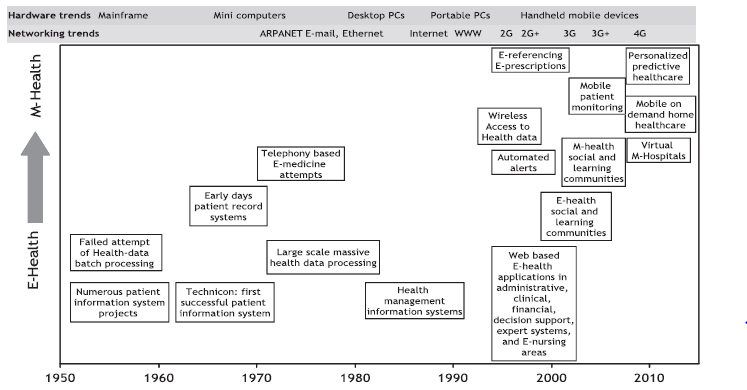
\includegraphics[width=\textwidth]{images/ehealth_evol.png}
\caption{Evolution over the time from the e-Health to the m-Health}
\label{fig:e2m_health}
\end{figure}

Wireless Sensor Network (WSN) is an emerging technology area based on the utilization of wireless gadgets to build a complete ICT-based wireless monitoring system. It consists of many nodes that can communicate with each other with routing responsibilities. Each node is equipped with a sensing unit, a memory, a microcontroller, a wireless communication interface and a power source.


The growing interest in the use of WSNs has been driven by the large number of emerging applications, such as home and industrial automation \cite{gomez2010wireless,akerberg2011future}, process monitoring \cite{zapater2012ubiquitous, khanna2012machine} and healthcare applications \cite{journals/jst/AbidoyeAAAN11, ko2010wireless, pawar2012framework}. They enable dense and flexible deployments at low cost.


One of the most promising uses of WSNs is the healthcare monitoring. It requires special wearable sensors placed on the  body surface. This peculiarity gives its name to the Wireless Body Sensor Network, in which spatially distributed sensors, each equipped with a radio transceiver --normally, Bluetooth or ZigBee ones \cite{chen2013review}--, cooperate with each other to monitor physiological or environmental human conditions. This kind of networks are usually integrated into a broader multitier telemedicine system \cite{Otto:2005:SAW:2010498.2010502, journals/jst/AbidoyeAAAN11, chen2013review, jovanov2011body, jovanov2009system}.


The amount of different types of measures currently provided by WBSNs is extensive:  electroencephalogram \cite{dilmaghani2011wireless}, stress \cite{jovanov2003stress}, emotions \cite{nasoz2004emotion}, blood pressure \cite{espina2006wireless} and accelerometry \cite{chung2008wireless} among others.



\section{Algorithms for wearable sensors in health monitoring systems}

As we have mentioned before, nowadays we are witnessing an increase in the development of wearable sensors for health monitoring systems. An important aspect of study in such systems is how the data gathered -in particular continuous time series measurements- are treated and processed. 

The integration and interpretation of the sensor signals usually pursue anomalies detection, prediction or decision making \cite{banaee2013data}. Therefore, the idea is to extract relevant medical information from large physiological data sets. Known in a wider context as \emph{data mining}, this intention normally becomes a computational process that involves artificial intelligence, machine learning, statistics and database systems.

The set of available methods and algorithms of data mining is very varied.The most common ones and their main characteristics and applications are listed below:

\begin{description}
	
	\item{\textbf{Support Vector Machines}\hfill \\
	The Support vector machines (SVM) technique is one of the main learning methods applied in classification and regression. Being primarily designed for two-class problems, the method derives some selected features from well known data and finds the optimal hyperplane -a linear classifier- to separate the unseen information into two classes in order to make a decision model \cite{cortes1995support}. 

	It is widely use for anomaly detection and decision making because of its ability to distinguish (non)healthy patterns. For instance, SVMs have been used to find out arrhythmia in ECG signals \cite{hu2008robust} and seizure episodes \cite{lee2012low}. 

	However, SVM is not an appropriate method to integrate domain knowledge and cannot be applied to find the unexpected information from unlabeled data.}

	\item {\textbf{Hidden Markov Models}\hfill \\
	A Markov Model is a stochastic process where it is assumed that the future states of a changing system depend only on the current one. In the Hidden Markov Models (HMM), some of these states are hidden from an observer in the sense that an observer cannot directly determine which state the system is in at any given point in time. However, a number of observable parameters dependent on the current state of the system are visible. Based on the visibility of this dependance, the occurrence probability of each state can be compute \cite{quwaider2008body}.

	HMM models are especially applied to temporal pattern recognition because of its ability for modeling sequential data. They have been used, for example, to detect abnormal values in blood glucose level \cite{zhu2011automatic} and perform a probabilistic segmentation for populating medical time series databases \cite{woodbridge2011salient}.}

	\item {\textbf{Artificial Neural Networks}\hfill \\
	Artificial Neural Networks (ANN) try to emulate the way in which biological neurons integrate and process the information of the brain. The basis of this technique lies on how the combination of the simple behaviour of each artificial neuron can result in a network with a much more complex performance. Thus, by applying different weights and non-linear functions to the input signals, the ANNs are able to model complex relationships where the correlation among the input parameters is not easily detectable \cite{al2011artificial}.

	ANNs are widely used for complex classification and prediction tasks in the medical domain. For instance, they have been used to assess the clinical quality of the pulses in PPG \cite{li2012dynamic} or to recognize heart rate variability patterns using ECG and accelerometer sensors \cite{vu2010online}. ANNs have also been proposed to predict blood glucose levels \cite{chatterjee2013persuasive}.}

	\item {\textbf{Decision Trees}\hfill \\
	Based on recursive data segmentation, decision trees provides an efficient representation of rule classification. During the process, the
	features of the input data are selected by descending order of robustness. That way, data is splitted by creating a tree-like model.

	This method has been proposed for the discrimination of emotional physiological signals evoked \cite{frantzidis2010classification}, for on-body heat stress risk prediction \cite{gaura2013leveraging}, and many other applications.

	Decision trees are simple and easy to implement.However, its efficiency worsen with the number of features to deal with, so these models are not usually applied to big and complex data.
	}

\end{description}

Other techniques widely used in diagnosis, prediction and decision making are Gaussian Mixture Models (GMM), Rule-Based Methods (RBM), Bayesian Networks (BN) and Self-Organizer Maps (SOM) among others \cite{banaee2013data, bellazzi2008predictive, fu2011review}. \figref{stateart_algorithms} extracted from \cite{banaee2013data} compare the mentioned methods and some others in terms of usage with different types of input signals.

\begin{figure}[!ht]
\centering
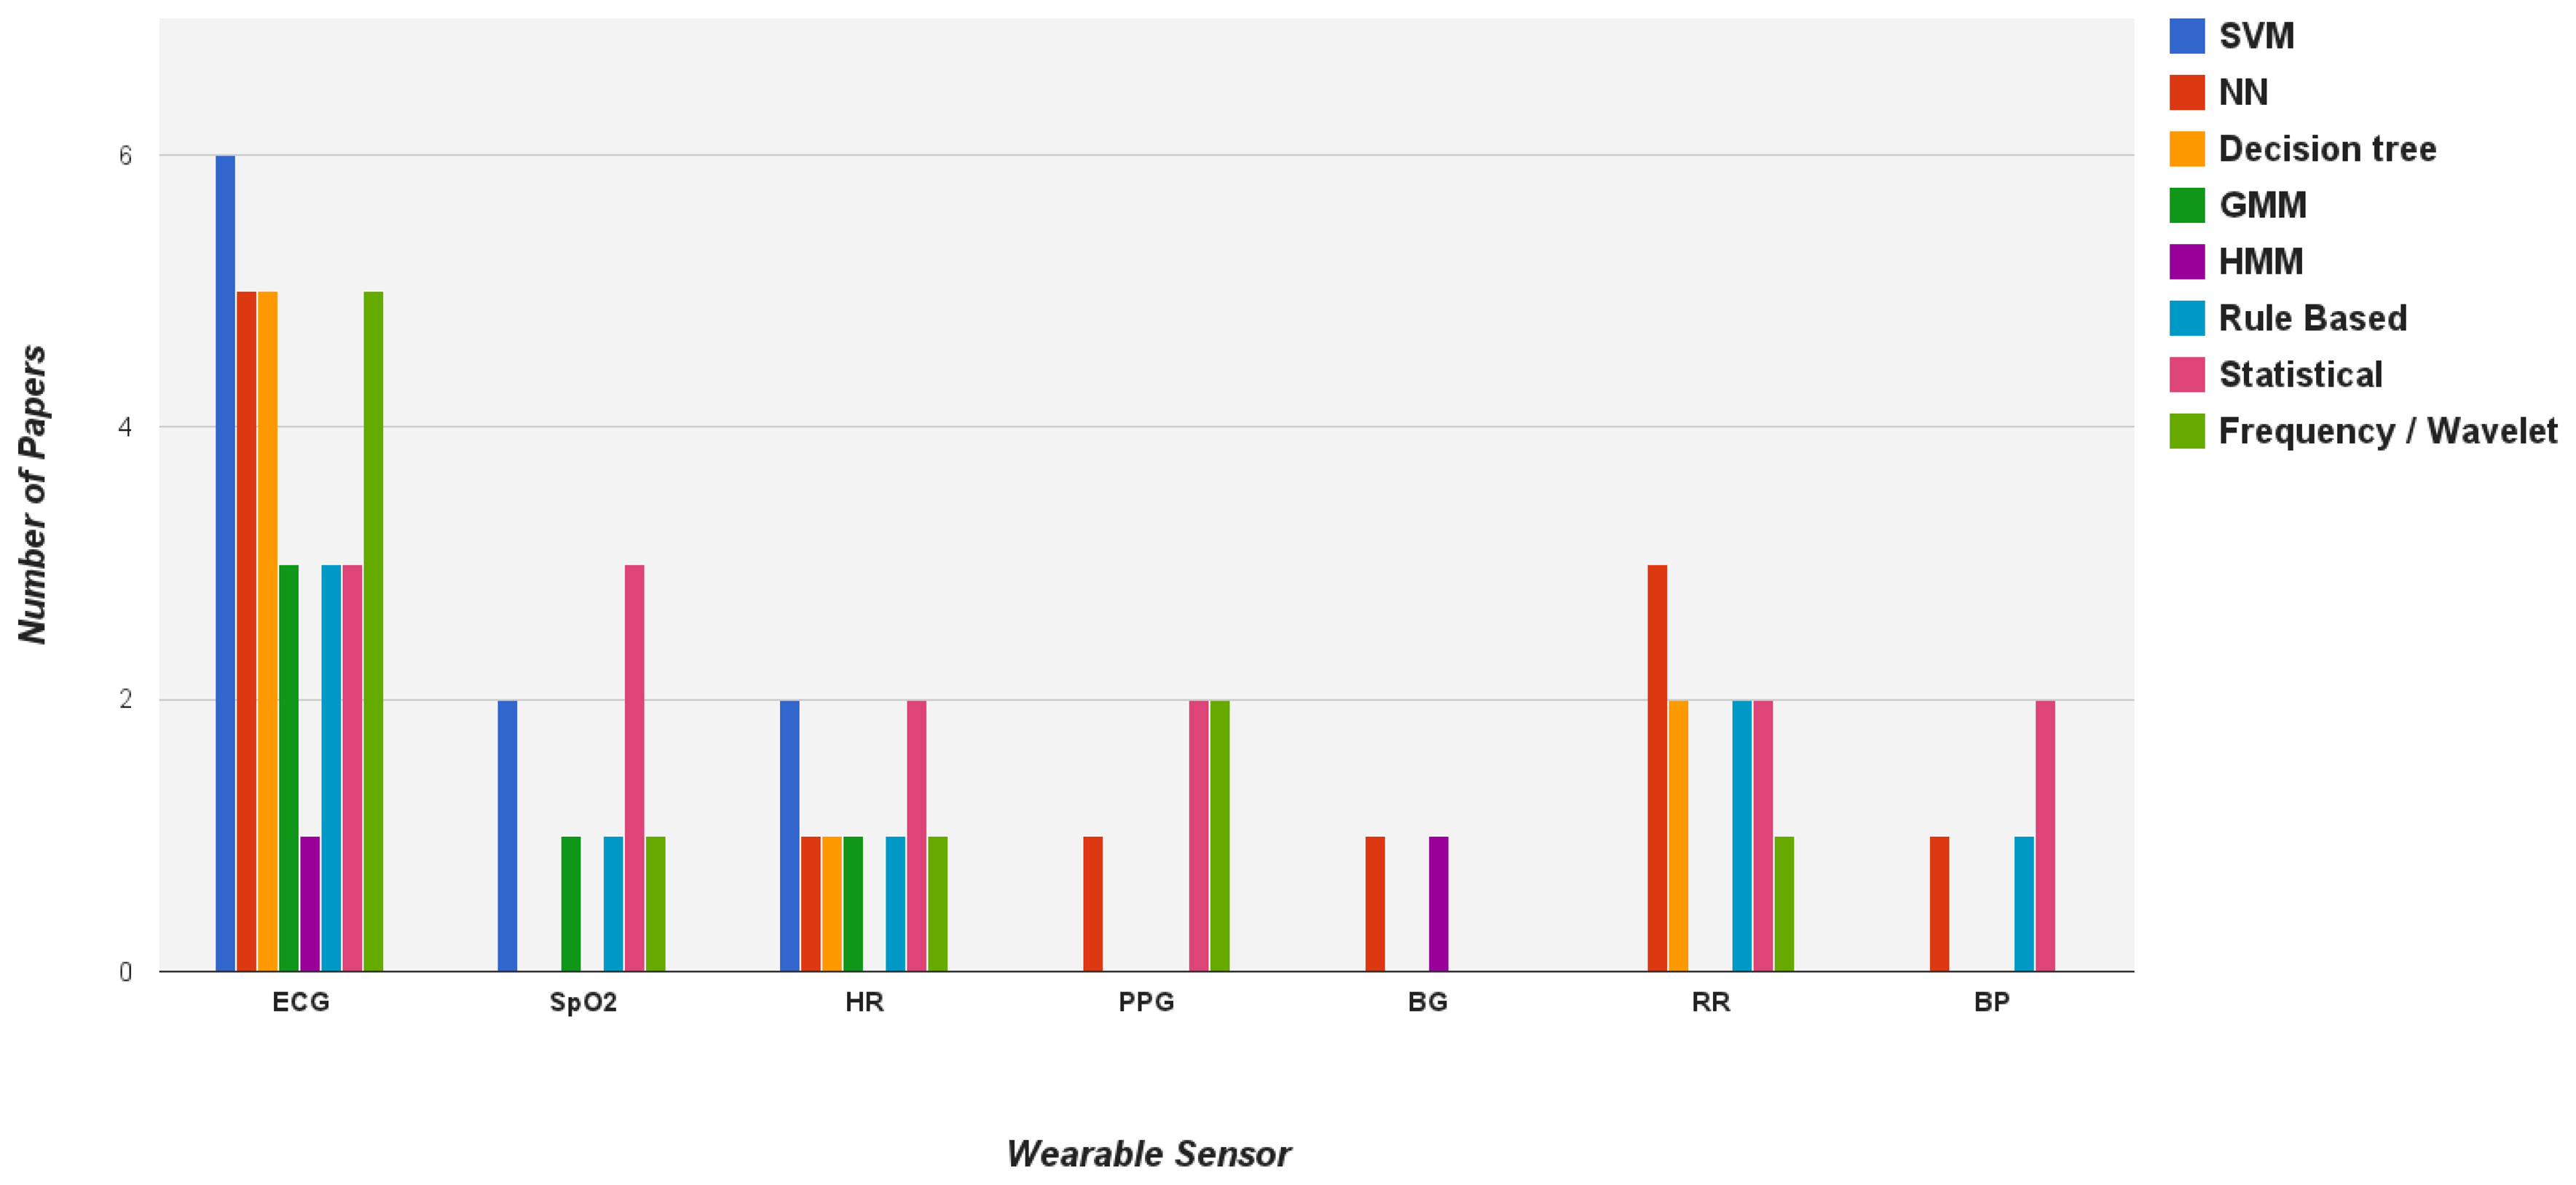
\includegraphics[width=\textwidth]{images/stateartalgorithms.png}
\caption{Comparison of some of the most common techniques used with physiological signals}
\label{fig:stateart_algorithms}
\end{figure}


% TEORIA
\chapter{Neural Networks}
\label{chapter:nn}

As we have mentioned in \charef{introduction}, our data mining approaches are based on Artificial Neural Networks (ANNs).
This kind of algorithm is currently the most popular data modeling method used in the medical domain because of its more than acceptable predictive performance. That is the reason why we opted in favour of ANNs for achieving  our final aim of predicting migraine crisis. 

In order to truly understand ANNs, it is necessary to have a minimum knowledge about those characteristics of brain function that have inspired the development of artificial neural networks
; \ie, how the neurons of the brain conduct themselves and interact each other.

\section{Biological Neural Networks}
%\section{Neural Networks}
\label{sec:BNN}

Neurons are nerve impulse-conducting cells that shape the nerves, the brain and the spinal column. They are considered as the functional unit of the nervous system. A typical neuron is divided into four regions: the soma or cell body, the axon, the dendrites and the synapses. The next lines try to describe very briefly the main characteristics and functions of each region and how they interact each other \cite{levitan2015neuron}. \figref{neuronstructure} shows how they are organized.

\begin{figure}[!ht]
\centering
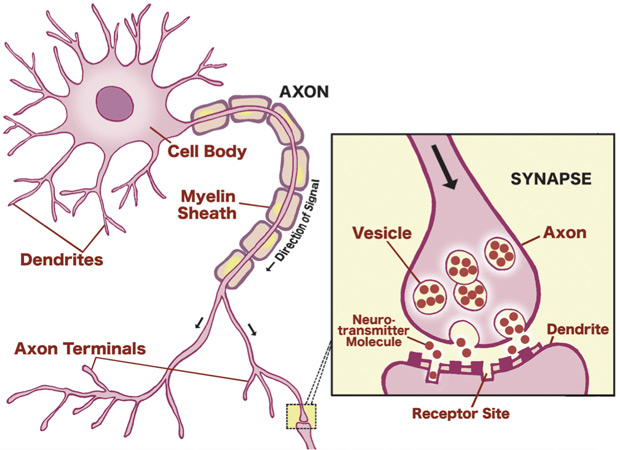
\includegraphics[width=0.6\textwidth]{images/neuronstructure.jpg}
\caption{Model of the structure of a neuron}
\label{fig:neuronstructure}
\end{figure}

The soma is the main part of the neuron in which the dendrites and the axon branch off of. It also contains the cell nucleus.Dendrites are thin structures that extend for hundreds of micrometres and branch multiple times shaping a complex ``dendritic tree''. An axon is a special cellular extension that travels for distances ranging from micrometers to meters before terminating.

The synapses are specialized regions or junctions that allows cell to cell connection for communicating. At the majority of synapses, a neuron receives information from other neurons through its dendrites. In the soma, the input signals are integrated and processed, and the axon is where the output signal is transmitted to a third neuron. This way, neurons can connect to each other to form neural networks.

The information that neurons exchange is electrical in nature, although the process is mediated by chemical substances. 
This way, axons are specialized for the conduction of a particular type of electric impulse called \emph{action potential}.
Then, the transmission of the information to a different neuron is carried out with the help of some biomolecules called neurotransmitters. 
This latter chemical process is called \emph{synapsis}. 
Thus, if a neuron $j$ sends a signal to neuron $i$, the former is called \emph{presynaptic} neuron and the latter is known as the \emph{postsynaptic} neuron. 
It is the arrangement of neurons and the strengths of the individual synapses, determined by the chemical
process of the neurotransmitters, that establishes the function of the neural network.

For the development of some ANNs algorithms, it is important to understand how an action potential is and conducts. We describe its mechanism in the following section.

\subsection{The action potential}
\label{subsec:actionpotential}
Every neuron is surrounded by positive and negative ions. 
The excess of negative charge in the inner surface of its membrane and the abundance of positive charge in the outer surface create a non-zero electric potential.

When a neuron is in the resting state, that is when it is not receiving any input signal, the electric potential across the axonal membrane is around $-60$mV to $-70$mV (the inside negative relative to the outside). When the neuron is stimulated, \ie, when it receives an input signal, some of the ion channels of the axon open and others close. This results in an electrical current that flows into del cell and the membrane potential of the axon becomes less negative.

If the electric disturbance is great enough and the electric potential reaches a determined threshold (approximately $-55$mV), a sudden change of voltage happens and the cell produces a electric spike known as action potential \cite{cellBiology}. 

An action potential consists on the following three phases. Firstly, the phenomenon called \emph{depolarization} during which the membrane potential changes exceed the critical value.
This depolarization of the membrane is followed by a rapid decrease in the value of the electric potential known as \emph{repolarization}.
Directly after, the membrane potential goes through a phase under the resting potential called \emph{hyperpolarization} and then slowly returns back to the resting potential.
These characteristics (see \figref{actionpotential}) distinguish an action potential from other types of changes in electric potential across the plasma membrane and allow an action potential to move along an axon without diminution. 

The action potentials are identical to each other, so it is the time between consecutive spikes what encodes the information transmitted. Related to this, it has to be noted that, there is a period of time called \emph{refractory period} during which a neuron is incapable of emitting a second spike. More precisely, this refractory period is the amount of time it takes for the excitable membrane of the neuron to be ready for a second stimulus.

\begin{figure}[!ht]
\centering
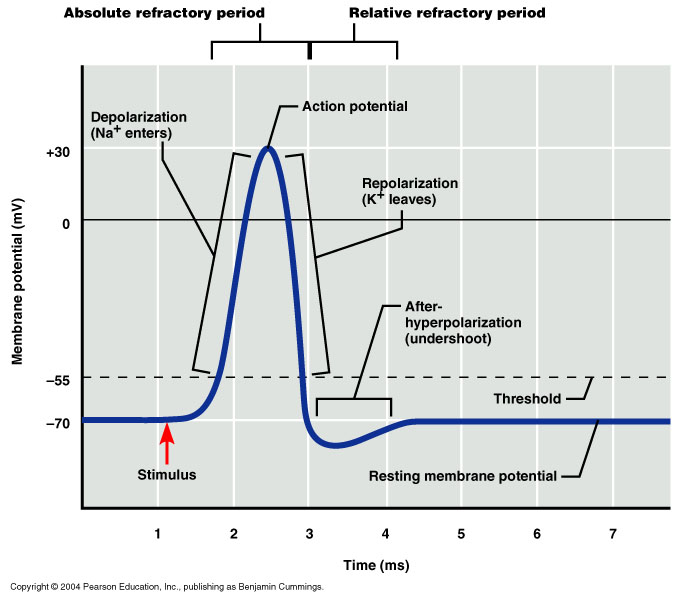
\includegraphics[width=0.7\textwidth]{images/actionpotential.jpg}
\caption{Schematic action potential and its main characteristics}
\label{fig:actionpotential}
\end{figure}


\section{Artificial Neural Networks}
%\section{Artificial Neural Networks}
\label{sec:ANN}
ANNs represent a type of computing based on the way that the brain performs computations. It does not approach the complexity of the brain; however, there are three similarities between biological and artificial neural networks: 

\begin{itemize}
	\item The basic unit of both systems -the neuron- is a very simple computational element that are highly interconnected.
	\item The connections among those neurons determine the function of the network.
	\item Despite having a very simple set of rules of behaviour, when a neuron interacts with others, the global response of the system becomes much more complex.
\end{itemize}

The next sections try to explain how a biological neuron is model in order to build artificial neural networks capable of solving complex problems.

\subsection{Neuron model}
\label{subsec:neuronmodel}

As described in \secref{BNN}, a typical biological neuron has four main regions: the soma, the axon, the dendrites and the synapses. These parts are also be differentiated in an artificial neuron. \figref{neuronmodel} shows how a biological neuron is model for ANNs.

\begin{figure}[!ht]
\centering
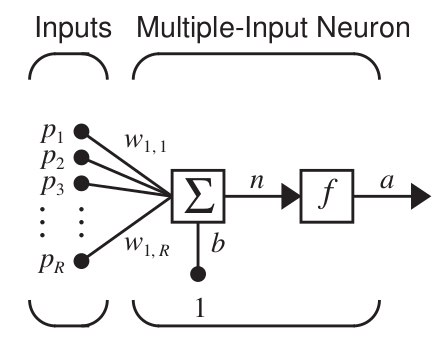
\includegraphics[width=0.5\textwidth]{images/neuronmodel.png}
\caption{Model of an artificial neuron inspired in a biological one}
\label{fig:neuronmodel}
\end{figure}

In an artificial neuron, the \emph{inputs} $p_{k}, k=1,...,R$ are multiplied by \emph{weights} $w_{k}$ and summed up together with the optional constant \emph{bias} or \emph{offset} term $b$. The resulting scalar $n$, often referred to as the \emph{net input}, goes into the \emph{activation function} -also called \emph{transfer function}- $f$, which produces the scalar neuron \emph{output} $a$.
Thus, the \emph{output} of the neuron $i$ becomes \cite{Demuth:2014:NND:2721661}:

\begin{equation}
a_{i}=f_{i}(n_{i})=f_{i}(\sum_{k=1}^R w_{ki}p_{k}+b_{i})
\label{eq:expandedgeneralneuroneq}
\end{equation}

Relating this neuron model back to the biological neuron that we discussed in \secref{BNN}, the set of \emph{inputs} $p_{k}$ correspond to the dendritic tree,
each \emph{weight} $w_{k}$ emulates the strength of a synapse, the soma is represented by the summation and the \emph{activation function} $f$,
and the neuron \emph{output} $y$ represents the signal on the axon.

The behave of the neuron depends strongly on the particular activation function that is chosen. Then the scalar parameters $w_{k}$ and $b$ will be adjusted by some learning rule so that the neuron input/output relationship meets some specific goal.

The activation function $f$ may be a linear or a nonlinear function of the net input $n$. 
A particular function is chosen to satisfy some specification of the problem that the neuron is attempting to solve. The following are some of the functions often used in ANNs \cite{Demuth:2014:NND:2721661}:

\begin{description}
	\item{\textbf{\emph{Hard limit} or \emph{Step} function}\hfill \\
	It sets the output of the neuron to 0 if the function argument is less than 0, or 1 if its argument is greater than or equal to 0. Its symetric version follows the expression:
		\begin{equation}
		a = f(n) =
  			\begin{cases}
    			-1 & \text{if } n < 0\\
    			1 & \text{if } n \geq 0
  			\end{cases}
		\label{eq:hardlimit}
		\end{equation}

	This activation function is commonly used to create neurons that classify inputs into two distinct categories.
	}
	\item{\textbf{\emph{Linear} function}\hfill \\
	The output of a linear transfer function is equal to its input ($a=f(n)=n$). This simple function have some variations that are often used in artificial neurons:
	\begin{itemize}
		\item \emph{Positive linear} function, which guarantees to take nonnegative values according to the equation:
		\begin{equation}
		a = f(n) =
  			\begin{cases}
    			0 & \text{if } n < 0\\
    			n & \text{if } n \geq 0
  			\end{cases}
		\label{eq:positivelinear}
		\end{equation}

		\item \emph{Saturating linear} function, whose symmetric version is mathematically expressed as:
		\begin{equation}
		a = f(n) =
  			\begin{cases}
    			-1 & \text{if } n < -1\\
    			n & \text{if } -1 \leq n \leq 1\\
    			1 & \text{if } n > 1
  			\end{cases}
		\label{eq:saturatinglinear}
		\end{equation}
	\end{itemize}
	}
	\item{\textbf{\emph{Log-Sigmoid} function}\hfill \\
	This activation function takes the input (which may have any value between plus and minus infinity) and squashes the output into the range 0 to 1, according to the expression:

	\begin{equation}
	a = f(n) = \frac{1}{1+e^{-n}}
	\label{eq:logsig}
	\end{equation}

	The log-sigmoid function is commonly used in multilayer networks that are trained using the backpropagation learning rule (see \secref{learningrules}), in part because this function is differentiable.
	}
	\item{\textbf{\emph{Hyperbolic Tangent Sigmoid} function}\hfill \\
	The hyperbolic tangent function produces positive numbers between -1 and 1 according to:
	\begin{equation}
	a = f(n) = \frac{e^{n}-e^{-n}}{e^{n}+e^{-n}}
	\label{eq:tansig}
	\end{equation}
	Because this function has a derivative, it can also be used with gradient descent based training methods as it is the backpropagation rule.
	}

\end{description}

\subsection{Neural network model}
\label{subsec:neuralnetworkmodel}

An ANN is then build by connecting several neurons.
Serial connections comprise different layers of neurons. 
Parallel connections increase the number of neurons in the same layer of the network.
The number of neurons in the last layer determines the number of outputs $S$ of the network. Thus, a huge amount of different topologies can be form. 

In addition to the activation function $f$, the number of inputs $R$ of each neuron can be configured, resulting in almost an infinite source of possible combinations with which try to solve any kind of scenario.
It must be noted that the activation functions are usually assumed to be the same in each layer of neurons. 
Normally a hyberbolic tangent or the sigmoid function is used, leading the ANN to a nonlinear parameterized map from input space $p\in\mathbb{R}^S$ to output space 
$a\in\mathbb{R}^R$.

\figref{neuralnetworkmodel} shows an example of an artificial neural network topology with three layers and the same number of neurons in each layer. 

\begin{figure}[!ht]
\centering
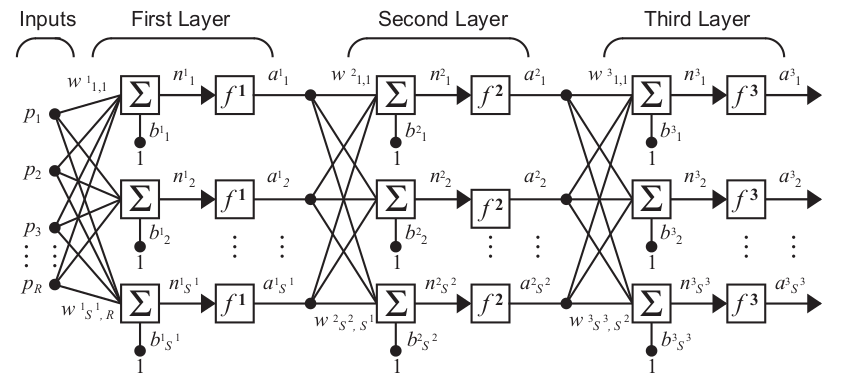
\includegraphics[width=\textwidth]{images/neuralnetworkmodel.png}
\caption{Model of three-layer Artificial Neural Network}
\label{fig:neuralnetworkmodel}
\end{figure}

Denoting
$\mathbf{p}$ as the $R\times 1$-dimensional input vector of the whole network, 
$\mathbf{b}^1$ the $S\times 1$-dimensional bias vector of the first layer and 
$\mathbf{W}^1$ as the $S\times R$-dimensional matrix of weights of the same layer, 
the $S\times 1$-dimensional net input vector of that particular layer $\mathbf{n}^1$ can be expressed as:
\begin{equation} 
\mathbf{n}^1=\mathbf{W}^1\mathbf{p}+\mathbf{b}^1
\label{eq:netinputvector}
\end{equation}

This way, \figref{neuralnetworkmodel} can we redrawn as \figref{neuralnetworkmodelVectorial} and, combining \esref{expandedgeneralneuroneq}{netinputvector}, the $S\times 1$-dimensional output vector of the whole network 
$\mathbf{a}^3$ can be written as:

\begin{equation}
\mathbf{a}^3=\mathbf{f}^3(\mathbf{W}^3\mathbf{f}^2(\mathbf{W}^2\mathbf{f}^1(\mathbf{W}^1\mathbf{p}+\mathbf{b}^1)+\mathbf{b}^2)+\mathbf{b}^3)
\label{eq:ouputnetworkvector}
\end{equation}

\begin{figure}[!ht]
\centering
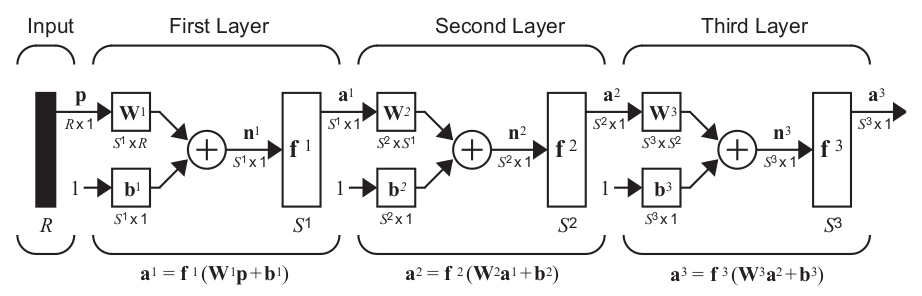
\includegraphics[width=\textwidth]{images/neuralnetworkmodelVectorial.png}
\caption{Model of three-layer Artificial Neural Network with matrix notation}
\label{fig:neuralnetworkmodelVectorial}
\end{figure}

It is important to highlight that, when implementing ANNs, the first layer is called \emph{input layer}, the last one \emph{output layer} and all the intermediate ones are known as \emph{hidden layers}. When there is no hidden layers, it is said that the net is a one-layer network. This way, two-layers networks will denote a net with a unique hidden layer. The reason of this is that the weigths of the input layer are usually fixed to $w=1$.

\subsection{Advantages and disadvantages}

\textsc{COPY-PASTE!!!!!!!!!!!!!!!!!!!!!!!!!!!! - ESCRIBIR}\\
Due to the admissible predictive performance of NN, it is presently the
most popular data modeling method used in the medical domain [37]. The ability of the NN is to model
highly nonlinear systems such as physiological records where the correlation of the input parameters is
not easily detectable [71].

In sum, since the progress of learning in NN would be complex, the method is commonly used for
decision making in clinical conditions with large and complicated data sets. But same as SVM it could
not handle domain knowledge to enrich the results. Additionally, as the modeling process in NN is a
black box progress, NN method needs to justify for each input data. So, NN is not counted as a portable
technique to easily apply for diverse data sets.

Artificial neural networks were up until recently the
most popular artificial intelligence-based data modeling
algorithm used in clinical medicine. This is probably due to
their good predictive performance, albeit they may have a
number of deficiencies [18] that include high sensitivity to the
parameters of the method—including those that determine
the architecture of the network, high computational cost in
training, and induction of the model that may – at best – be
hard to interpret by domain experts. Neural networks may be
able to model complex non-linear relationships, comprising
an advantage over simpler modeling methods like the na ̈ve
ı
Bayesian classifier or logistic regression.
}

\section{Topologies of Artificial Neural Networks}
\label{sec:topologies}

There is a wide set of ANNs architectures.
Since our final aim is to forecast a time series,
the following sections are focused on those network topologies suitable for this purpose. 
Nonetheless, in order to better understand the building process of each architecture, we explain firstly the \emph{Perceptron} topology, which is the simplest structure.

	\subsection{Perceptron}
	
\label{subsec:ANN:perceptron}

Perceptrons are the simplest topology we can build with artificial neurons. 
Nevertheless, the knowledge of the operations behind perceptrons provides a good
basis for understanding more complex networks.

A perceptron neuron uses the hard-limit activation function, which produces a 1 if the net input is equal to or greater than 0; otherwise it produces a 0. 
This function gives a perceptron the ability to classify input vectors by dividing the input space into two regions, which are formed by the decision boundary line L at $\mathbf{Wp} + b = 0$ \cite{demuth2008neural}. 
This line is perpendicular to the weight matrix W and shifted according to the bias b 
(notice that hard-limit neurons without a bias will always have a classification line going through the origin).

As shown in \figref{perceptron}, the perceptron network consists of a single layer of 
$S$ perceptron neurons connected to $R$ inputs through a set of weights $\mathbf{W}$.

\begin{figure}[!ht]
\centering
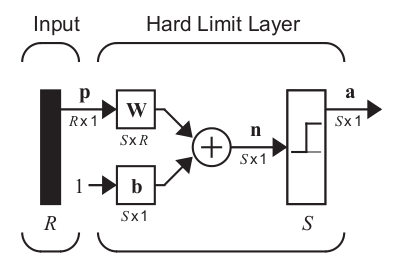
\includegraphics[width=0.5\textwidth]{images/perceptron.png}
\caption{Perceptron network}
\label{fig:perceptron}
\end{figure}




	\subsection{Time Delay Neural Networks}
	
\label{subsec:ANN:TDNN}

Prediction requires the use of dynamic neural networks, as discussed in
Chapter 14. The specific form of the network will depend on the particular
application. The simplest network for nonlinear prediction is the focused
time-delay neural network, which is shown in Figure 22.3. This is part of a
general class of dynamic networks, called focused networks, in which the
dynamics appear only at the input layer of a static multilayer feedforward
network. This network has the advantage that it can be trained using static
backpropagation algorithms, since the tapped-delay-line at the input of the
network can be replaced with an extended vector of delayed values of the
input.

\begin{figure}[!ht]
\centering
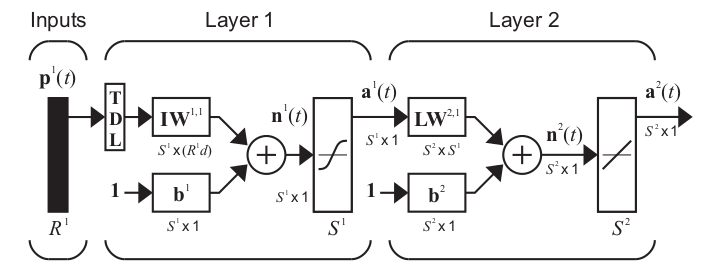
\includegraphics[width=0.5\textwidth]{images/tdnn.png}
\caption{Time Delay network}
\label{fig:tdnn}
\end{figure}

	\subsection{Non-Linear Autorregresive with Exogenus Input}
	
\label{subsec:ANN:NARX}

The nonlinear autoregressive network with exogenous inputs (NARX) is a
recurrent dynamic network; \ie, it has feedback connections.  Based on
the linear ARX models, NARX ones have been demonstrated suitable for
modeling nonlinear systems and specially time series.

The simplest NARX network consists on a feedforward neural network
with a first TDL at the input plus a delayed connection from the
output to the input layer (a second TDL).
\figref{narx} shows a schematic version of this NARX network.

\begin{figure}[!ht]
\centering
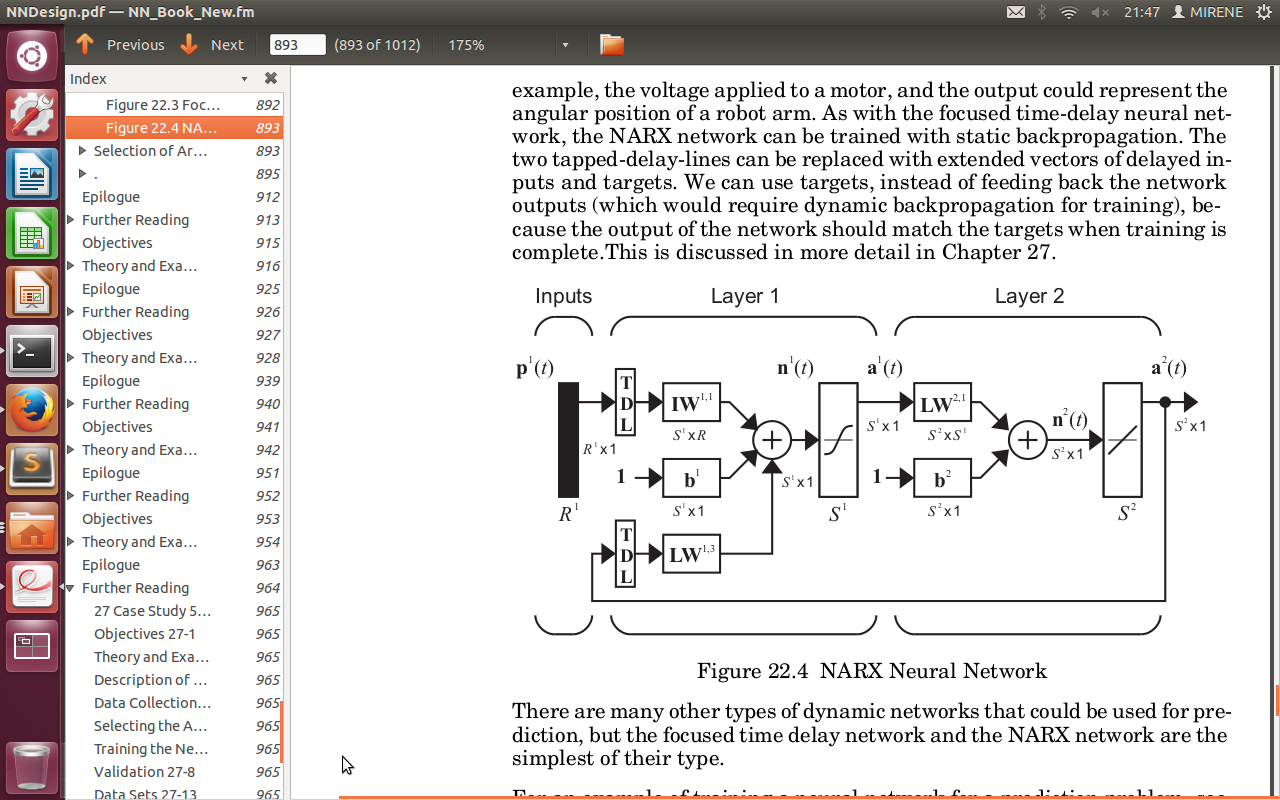
\includegraphics[width=\textwidth]{images/narx.png}
\caption{NARX network}
\label{fig:narx}
\end{figure}

The defining general equation of an one-step-ahead ARX model is
% \begin{equation}
% \begin{split}
% y(t) =f(y(t-1),y(t-2),...,y(t-n_{y}), \\
% u(t-n_{k}),u(t-(n_{k}+1)),...,u(t-(n_{k}+n_{u})))
% \end{split}
% \end{equation}
\begin{equation}
\hat{y}(t) =f(\hat{y}(t-1),\hat{y}(t-2),...,\hat{y}(t-d_{y}), u(t-1),u(t-2),...,u(t-d_{u}))
\label{eq:narxequation}
\end{equation}
where the value of the dependent output signal $\hat{y}(t)$ is
regressed on the $d_{y}\geq1$ previous values of the same output
signal and $d_{u}\geq0$ previous values of the independent exogenous
input signal $u(t)$ \cite{lin1996learning}.  The unique dissimilarity
between ARX and NARX models lies in the linearity of the function $f$.
Thus, in the NARX neural network of \figref{narx}, $f$ is a
combination of the non-linear activation functions $\mathbf{f}^1$ and
$\mathbf{f}^2$.

%The prediction horizon $n_{k}$ is defined as the shift among corresponding input and output values so that current input is used for predicting the output in $n_{k}$ time steps in the future.

In what concerns training a NARX network the
named \emph{Backpropagation Through Time} version of the
backpropagation algorithm can be used (read \subsecref{bptt}). The
process can be carried out in one out of the two modes shown
in \figref{narxtrainingarch} \cite{menezes2008long}:
\begin{itemize}
	\item Parallel architecture, where the output $\hat{y}(t)$ is
	fed back to the input of the feedforward neural network as
	part of the standard NARX architecture.  

        \item Series-parallel architecture, in which the true output
	$y(t)$ -well-known target output- is used instead of feeding
	back the estimated output $\hat{y}(t)$.
\end{itemize}

Idially, NARX networks are trained with the series-parallel architecture and tested with the only parallel one.

\begin{figure}[!ht]
\centering
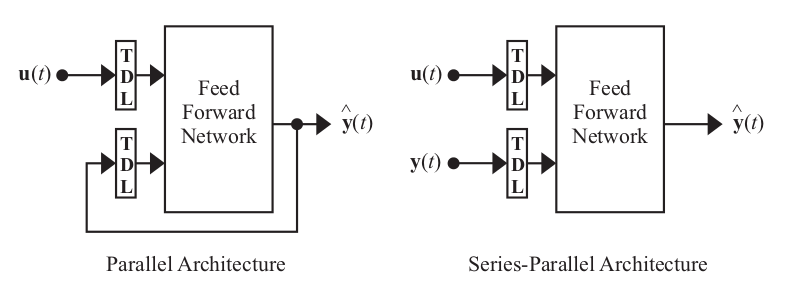
\includegraphics[width=\textwidth]{images/narxTrainingArchitectures.png}
\caption{NARX network training architectures}
\label{fig:narxtrainingarch}
\end{figure}




	\subsection{Spiking Neural Networks}
	%\section{Artificial Neural Networks}
%\subsection{Spiking Neural Networks}
\label{sec:ANN:SNN}
\section{The backpropagation learning algorithm}

\label{sec:generalbackprop}

Backpropagation is a gradient-descent supervised learning algorithm 
in which the combination of weights that minimizes a given error function is considered to be a solution of the learning problem. It is suitable for both static and dynamic ANNs.

Generally speaking, a network represents a chain of function compositions which transform an input to an output vector. Each initialization of a network is a particular implementation
of that composite function. Thus, the learning problem consists of finding the optimal combination of weights so that the particular network function approximates a given function as closely as possible. However, the target function is a priori unknown; we only have some matching patterns.

As we explained in \subsecref{learningrules} when talking about supervised learning algorithms, the just mentioned patterns comprise our training set. Lets assume we are given a training set defined by $\{\mathbf{p_{1}} , \mathbf{t_{1}} \}, \{\mathbf{p_{2}} , \mathbf{t_{2}}\}, ...,
 \{\mathbf{p_{Q}} , \mathbf{t_{Q}} \}$
consisting of $Q$ ordered pairs of input $\mathbf{p}$ and target output $\mathbf{t}$ vectors.
At the beginning, 
when the input pattern $\mathbf{p}_{q}$ from the training set is presented to the neural network,
it produces an output vector $\mathbf{o}_{q}$ different in general from the target $\mathbf{t}_{q}$.
Hence, the final objective is to make $\mathbf{o}_{q}$ as equal as possible to $\mathbf{t}_{q}$ for $1 \leq q \leq Q$, which is possible by minimizing the error function of the network defined as
\begin{equation}
E=\frac{1}{2}\sum_{q=1}^{Q}
\parallel \mathbf{t}_{q}-\mathbf{o}_{q} \parallel^2
\label{eq:globalerrorfunction}
\end{equation}

Since this minimization process requires the computation of the gradient of the error function at each iteration step,
we must guarantee the continuity and differentiability of the error function.
In view of the algorithm computes only function compositions, 
the foregoing is traduced in the usage of a kind of activation function that accomplished the characteristics of continuity and differentiability. 
Some examples of suitable activation functions are: 
the linear function, taking care in its variants to avoid the points where the derivative is undefined; 
the log-sigmoid and the hyperbolic tangent sigmoid functions. 
On the contrary, the hard-limit will be an instance of a non suitable function.

After minimizing the error function for the training set, 
new unknown input patterns are presented to the network. 
The expected behaviour of the network is being capable to interpolate; 
\ie, recognize whether the new input vector is similar to a learned pattern 
and, accordingly, produce the corresponding similar output.

The backpropagation algorithm is threfore used to find a local minimum of the error function. 
To do this, the network parameters are firstly initialized with a random function. 
Then, the gradient of the error function is recursively computed and
used to correct the initial weights.

Next sections explained the rules of the backpropagation algorithm as well as the necessary modifications for its usage in the different architectures of ANNs described in \secref{topologies}.

\subsection{Static backpropagation algorithm}
\label{subsec:staticbackprop}
The static backpropagation is suitable for feedforward neural networks such as those introduced in \subsecref{neuralnetworkmodel}. For an accurate explanation of the learning rules behind this training algorithm, lets imagine a multilayer network with one input layer, an indetermined number of hidden layers and one output layer.

In a given time, the connection between the neuron $j$ of the $l$-th layer and the neuron $i$ of the $(l-1)$-th layer has a weight value of $w_{ji}$. The output $a$ of neuron $j$ for the input pattern $\mathbf{p}_{q}$ can be expressed in terms of the net input $n$ and the connection weights as follows
\begin{equation}
a_{qj}=f_{j}(n_{qj})=f_{j}(\sum_{i\in \Gamma_{j}}w_{ji}a_{qi})
\label{eq:neuronjoutput}
\end{equation}
where $\Gamma_{j}$ denotes the set of presynaptic neurons of the postsynaptic neuron $j$.

What is really intended is to compute the gradient of the error function. 
Since the weights are the parameters we can modify in order to produce the correct network output, 
this gradient is defined by the partial derivative with respect to the weights of the connections between the corresponding neurons. Hence, for each pattern $q$, the gradient of the error function evaluated in neuron $j$ is
\begin{equation}
\frac{\partial E_{q}}{\partial w_{qji}}
\label{eq:gradienterrorfunction}
\end{equation}

With \eref{neuronjoutput} and making use of the chain rule, Expression \ref{eq:gradienterrorfunction} can be transformed into
\begin{equation}
\frac{\partial E_{q}}{\partial w_{qji}}=
\frac{\partial E_{q}}{\partial n_{qj}}
\frac{\partial n_{qj}}{\partial w_{qji}}=
\frac{\partial E_{q}}{\partial n_{qj}} a_{qj}=
-\delta_{qj} a_{qj}
\label{eq:chainrulegradienterrorfunction}
\end{equation}
where $\delta_{qj}$ is a variable introduced just for a matter of notation.

Analising the sign of the above equation, two cases can be distinguished:
\begin{itemize}

\item If $\delta_{qj}a_{qj}<0$, the gradient of the error function is positive, which means that $E_{q}$ increases (decreases) when $w_{ji}$ rises (falls). In view of this, for getting a lower value of $E_{q}$ we only have to reduce the value of $w_{ji}$ in a controled way. The manner in which backpropagation update the weight value is by adding it the negative amount of $\delta_{qj}a_{qj}$ (remember that $\delta_{qj}a_{qj}<0$ in this case) multiplied by the constant $\eta$. This latter parameter is known as the \emph{learning rate of the algorithm} and it controls how big/small is the amount added to $w_{ji}$. 

\item The same reasoning is applied whether $\delta_{qj}a_{qj}>0$. In this case, $E_{q}$ decreases when $w_{ji}$ rises. The updated value of $w_{ji}$ can be therefore obtained by adding it the positive amount of $\delta_{qj}a_{qj}$ multiplied again by $\eta$.

\end{itemize}

Thus, the updating process of each weight $w_{ji}$ can be expressed mathematically as
\begin{equation}
w_{ji}\leftarrow w_{ji}+ \eta\delta_{qj}a_{qj}
\label{eq:updatingrule}
\end{equation}

The remainder is know how obtain the $\delta_{qj}$. Using the chain rule again and the first part of \eref{neuronjoutput}, we can expressed the mentioned term as
\begin{equation}
\delta_{qj}= 
- \frac{\partial E_{q}}{\partial n_{qj}}=
- \frac{\partial E_{q}}{\partial a_{qj}}
\frac{\partial a_{q}}{\partial n_{qj}}
\label{eq:factordelta}
\end{equation}

Since $a_{j}=f_{j}(n_{j})$, then
\begin{equation}
\frac{\partial a_{q}}{\partial n_{qj}}=
f_{j}'(n_{j})
\label{eq:factoractivationfunction}
\end{equation}
and only the first factor of the right part of \eref{factordelta} lasts. 

For its calculation, it is necessary to distinguished two situations:
\begin{itemize} 
\item If $j$ is an output-layer neuron, assuming that the output space is S-dimensional (\ie, $\in\mathbb{R}^S$), the output layer of the feedforward NN will be comprised by S neurons. Thus, \eref{globalerrorfunction} can be rewritten, for each pair $q$ of target-output vectors, as 
\begin{equation}
E_{q}=\frac{1}{2}\sum_{j=1}^{S} (t_{qj}-o_{qj})^2
\label{eq:patternerrorfunction}
\end{equation}

This way, and knowing that in this case $a_{j}=o_{qj}$ where $o$ denotes the output of the whole network, it is accomplished that
\begin{equation}
-\frac{\partial E_{q}}{\partial a_{qj}} =
-\frac{1}{2}\frac{\partial o_{qj}}{\partial}
\sum_{j=1}^{S} (t_{qj}-o_{qj})^2 =
...= t_{qj}-o_{qj}
\label{eq:factortarout}
\end{equation}

Finally, combining Equations \ref{eq:factordelta}, \ref{eq:factoractivationfunction} and \ref{eq:factortarout} we obtain
\begin{equation}
\delta_{qj}= f_{j}'(n_{j})(t_{qj}-o_{qj})
\label{eq:deltajoutput}
\end{equation}


\item If $j$ is not an ouput-layer neuron, then there will be a neuron $k$ in the $(l+1)$-th layer with a net input $n_{qk}$ when the pattern $q$ is presented to the network. Hence,
\begin{equation}
\frac{\partial E_{q}}{\partial a_{qj}}=
\sum_{j\in \Gamma_{k}}
\frac{\partial E_{q}}{\partial n_{qk}}
\frac{\partial n_{qk}}{\partial a_{qj}}=
\sum_{j\in \Gamma_{k}}
\frac{\partial E_{q}}{\partial n_{qk}}
\frac{\partial}{\partial a_{pj}}
\sum_{i\in \Gamma_{j}}w_{ji}a_{qi}= 
-\sum_{j\in \Gamma_{k}}\delta_{qk}w_{ji}
\label{eq:factorbackpropagated}
\end{equation}

Finally, combining Equations \ref{eq:factordelta}, \ref{eq:factoractivationfunction} and \ref{eq:factorbackpropagated} we obtain
\begin{equation}
\delta_{qj}= f_{j}'(n_{j})
\sum_{j\in \Gamma_{k}}\delta_{qk}w_{ji}
\label{eq:deltajNOoutput}
\end{equation}

\end{itemize}

The idea of the backpropagation algorithm is to update recursively each weight term.
Therefore, the steps to follow and repeat until the error function reaches a minimum are:
\begin{enumerate}
\item Present an input pattern $\mathbf{p}_{q}$ and calculate the error function with the network output $\mathbf{o}_{q}$ and the target $\mathbf{t}_{q}$ vectors with \eref{patternerrorfunction}.
\item Obtain the output $a_{qj}$ of each neuron $j$ of the network making use of \eref{neuronjoutput}.
\item Update each weight term with the rule of \eref{updatingrule}, where the $\delta_{qj}$ term follows \eref{deltajoutput} in case of an output-layer neuron and \eref{deltajNOoutput} it is a hidden-layer neuron.
\end{enumerate}


\subsubsection{Convergence}
\label{subsubsec:backpropconvergence}
???????????


\subsection{Backpropagation through time}
\label{subsec:bptt}
Backpropagation through time (BPTT) is a variant of the above backpropagation algorithm. While the latter is used to train static feedforward networks, the BPTT is suitable for dynamic neural networks.

\subsection{Backpropagation for spiking neural networks}
\label{subsec:snnbackprop}


% ADQUISICION SEÑALES
\chapter{Data acquisition}

\label{chapter:setup}
Before having deployed our WBSN system we had to have a minimum knowledge about the physiological signals we intended to monitor. The following lines describe briefly all the signals we monitored from the patients, as well as those other secondary variables we obtained from the formers. Then, we present the system we used to acquire the desired variables, as well as the procedure conducted with the patients.
\section{Physiological signals}

%\chapter{Experimental setup}
\label{sec:setup:phys-signals}

The clinical symptoms of migraine are widely accepted to be related to
the autonomic nervous system (ANS) \cite{melek2007autonomic,
sanya2005impairment, barbanti2013dopaminergic, gass2013autonomic,
becker2013premonitory, hassinger1999cardiovascular}. In contrast to
the somatic nervous system, which provides voluntary control of the
body, the ANS is the part of the peripheral nervous system that
controls visceral functions, acting largely below the level of
consciousness. Consequently, the ANS controls vital signs including
heart rate, digestion, respiration rate, vomiting and swallowing.


In the migraine disease, the involvement of the ANS is materialized in
a dysfunction in the regulation of the circulatory system and the
autonomic balance. As described in \cite{mendes2009assessing}, there
are several biometric variables that allow to assess changes in ANS
activity. Some of them and others have already been studied in
migraineurs: electrocardiogram (ECG) \cite{melek2007autonomic,
aygun2003electrocardiographic}, heart rate \cite{pmid23853566,
pmid19925627}, skin temperature \cite{zaproudina2013acral,
ordas2013increase}, blood pressure \cite{pietrini2005hypertension,
pmid19925627} and electroencephalogram
(EEG) \cite{bjork2011initiates}. The system used was able to register
all these signals and two more variables: oxygen saturation and
sweating, monitored as electrodermal activity. Both, oxygen saturation
and sweating, are related to the ANS too.

The main characteristics of the above-mentioned physiological signals
are described below.

\subsection{Electrocardiogram}
\label{subsec:setup:phys-signals:ecg}

An electrocardiogram (ECG) describes the electrical impulses that
travel through the heart. It provides information about the rate,
rhythm, and morphology of the heart.

\begin{figure}[!ht]
\centering
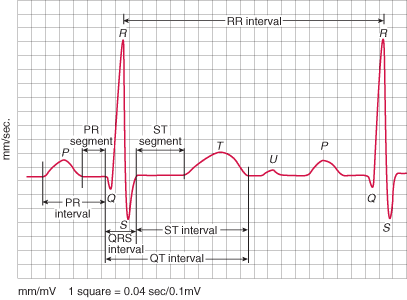
\includegraphics[width=0.8\textwidth]{images/ECGwave.png}
\caption{ECG wave}
\label{fig:ecg}
\end{figure}


A typical ECG wave of a normal heartbeat is described
in \cite{wang2008analysis}. It consists of a P wave, a QRS complex,
and a T wave as shown in \figref{ecg}. The first wave reflects the
sequential depolarization of the right and left atria. It usually has
positive polarity, and its duration is less than 120 milliseconds. The
spectral characteristic of a normal P wave is usually considered to be
low frequency, below 10–15 Hz. The QRS complex corresponds to the
depolarization of the right and left ventricles. It lasts for about
70–110 milliseconds in a normal heartbeat, and has the largest
amplitude of the ECG waveforms. Due to its steep slopes, the frequency
content of the QRS complex is considerably higher than that of the
other ECG waves, and is mostly concentrated in the interval of 10–40
Hz. The T wave reflects ventricular repolarization and extends about
300 milliseconds after the QRS complex. The position of the T wave is
strongly dependent on heart rate, becoming narrower and closer to the
QRS complex at rapid rates.


Normally, ECG is recorded by attaching a set of electrodes on the
chest, neck, arms, and legs.


\subsection{Pulse oximetry and plesthymographic curve}
\label{subsec:setup:phys-signals:ppg}


The pulse oximetry offers real-time assessment of oxygenation status
on a moment-to-moment basis. The foundation for pulse oximetry is the
spectral analysis: the detection and quantitation of oxygenated and
deoxygenated (or reduced) hemoglobin by their unique light absorption
characteristics \cite{sinex1999pulse, bagha2011real}.

\begin{figure}[!ht]
\centering
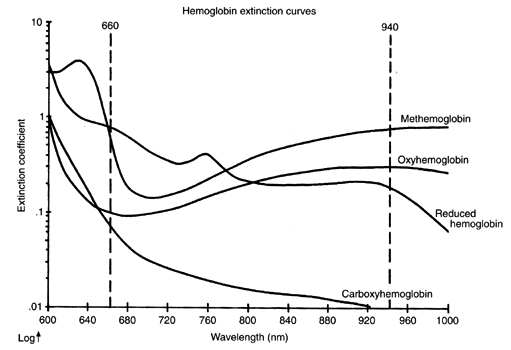
\includegraphics[width=0.9\textwidth]{images/hemoglobin.png}
\caption{Absorption of the red and the infrared lights by oxygenated and reduced hemoglobin}
\label{fig:hemoglobin}
\end{figure}



Two LEDs in the pulse oximeter emit light of specific wavelength
through a cutaneous vascular bed. A photodiode detector at the far
side measures the intensity of transmitted light at each wavelength,
from which oxygen saturation (SpO2) can be
derived \cite{bagha2011real}. \figref{hemoglobin} shows how oxygenated
hemoglobin absorbs more infrared light (910 nm) and allows more red
light (660 nm) to pass through, whereas reduced hemoglobin absorbs
more red light and allows more infrared light to pass through.


In the process of determining SpO2, the pulse oximeter functions as a
photoelectric plethysmograph. In this role, it measures changes in the
light absorption of the vascular bed. The resulting photoplesthymogram
(PPG) comprises a pulsatile physiological waveform attributed to
cardiac synchronous changes in the blood volume with each
heartbeat \cite{allen2007photoplethysmography}. This signal, shown
in \figref{bloodpressure}, is superimposed on a slowly varying
baseline with various lower frequency components attributed to
respiration, sympathetic nervous system activity and
thermoregulation. \figref{PPGnatvars} shows a complete picture of the
PPG waveform.

\begin{figure}[!ht]
\centering
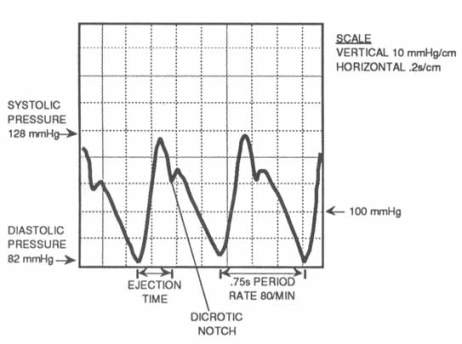
\includegraphics[width=0.8\textwidth]{images/BloodPressureWaveform.jpg}
\caption{Cardiac synchronous changes in the blood volume}
\label{fig:bloodpressure}
\end{figure}


\begin{figure}[!ht]
\centering
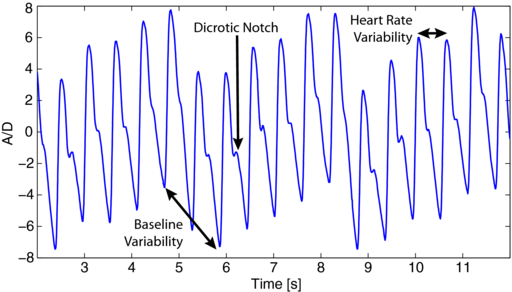
\includegraphics[width=0.8\textwidth]{images/PPGnaturalVariations.jpg}
\caption{PPG waveform}
\label{fig:PPGnatvars}
\end{figure}



Pulse oximetry is usually measured on skin surfaces with high
capillarity, such as that of the digits or the ear lobe.


\subsection{Heart rate}
\label{subsec:setup:phys-signals:hr}

The heart rate (HR) refers to the number of beats that the heart
performs in a time interval. It is usually expressed in beats per
minute.

ECG and PPG can be sources of instantaneous HR information, since both
signals present synchronous changes with each cardiac beat. In the
first case, HR is calculated through R-R intervals. In the PPG curve,
we can consider as the reference point the one in which the amplitude
of the waveform is maximum. Then, HR can be obtained from the time
interval existing between two consecutive reference
points. \figref{HRcalculus} shows these ECG and PPG parameters related
to the HR calculus.


\begin{figure}[!ht]
\centering
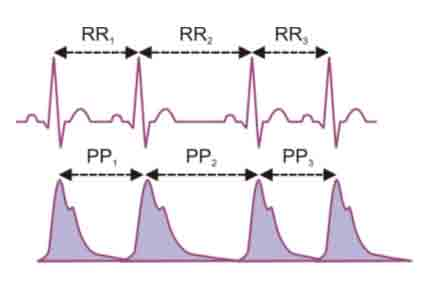
\includegraphics[width=0.6\textwidth]{images/PPGandECG.jpg}
\caption{ECG and PPG parameters related to the HR calculus}
\label{fig:HRcalculus}
\end{figure}


% \subsubsection{Blood pressure and pulse transit time}

% The pressure pulse generated by ventricular ejection is propagated through the arterial tree. The propagation velocity is determined by the elastic and geometric properties of the arterial wall and the blood density. Blood pressure (BP) is a commonly used parameter which carries important information about the status of the cardiovascular system.

% The measurement of pulse wave velocity (PWV), which is inversely related to arterial wall distensibility, offers a simple and potentially useful approach to measure the BP. Pulse transit time (PTT), defined as the time interval between the peak time of the R wave (ECG signal) and the time when pulse waveforms reach their maximum value (PPG signal), is one of the most common proposals for the non-invasive PWV estimation. Figure \ref{fig:PTTdet} shows this relationship among ECG, PPG and PTT.

% The explanation of how PTT and BP relate to each other is described in detail in \cite{choi2004evaluation, wong2005effects}.

% Since the PTT signal represents the time needed by a pulse wave to exit the heart and reach the place where PPG is measured, the larger the distance between that place and the heart, the lesser impact measurement error will have on the PTT determination. For this reason the pulse wave is usually detected at the fingertip \cite{hey2009continuous}.In this project, we will make use of the direct correlation between the PPG curve, the ECG curve and the BP estimation through PTT. However, we will avoid to work with absolute values of BP that would require the validation of the measure for every patient.

% \begin{figure}[!ht]
% \centering
% 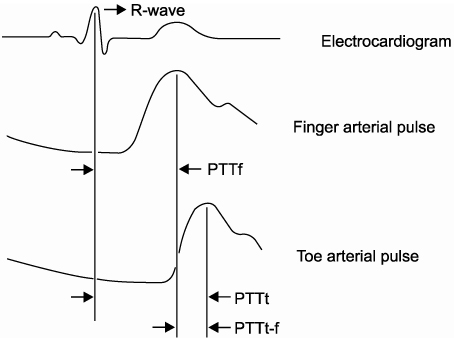
\includegraphics[width=0.8\textwidth]{img/PTT.jpg}
% \caption{Relationship among ECG, PPG and PTT}
% \label{fig:PTTdet}
% \end{figure}


\subsection{Electroencephalogram}
\label{subsec:setup:phys-signals:eeg}

An electroencephalogram (EEG) describes the electrical activity of the
brain generated by the cooperative and synchronous action of its
cells. The main characteristics of an EEG \figref{EEGrhythms}) are
described below \cite{blinowska2006eeg}.
\begin{itemize}

	\item It can be measured by means of electrodes placed on the
	scalp or directly on the cortex.

	\item The amplitude of an EEG of a normal subject in the awake
	state recorded with the scalp electrodes is 10–100 mV, whereas
	amplitudes are in the range 500–1500 mV, in the cortex.

	\item We can distinguish several rhythms in a EEG: delta
	(0.5–4 Hz), theta (4–8 Hz), alpha (8–13 Hz), beta (13–30 Hz),
	and gamma (above 30 Hz). Gamma components are difficult to
	record by scalp electrodes, and their frequency does not
	exceed 45 Hz. The contribution of different rhythms to the EEG
	depends on the age and behavioral state of the subject, mainly
	the level of alertness.
\end{itemize}

\begin{figure}[!ht]
\centering
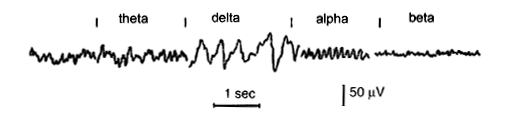
\includegraphics[width=\textwidth]{images/EEGrhythms.png}
\caption{EEG rhythms and amplitudes}
\label{fig:EEGrhythms}
\end{figure}



\subsection{Skin temperature}
\label{subsec:setup:phys-signals:temp}

Since the human skin forms the interface between the human body and
the thermal environment, skin temperature describes heat
transfer. Thermocouples, thermistors, and infrared sensors are the
thermally sensitive components generally applied for this
purpose \cite{van2006evaluation}.


\subsection{Sweating}
\label{subsec:setup:phys-signals:eda}

The human skin displays several forms of bioelectric phenomena,
especially in areas of the extremities such as the fingers, palms of
the hands, and soles of the feet \cite{PoligraphLesson}. The terms
galvanic skin resistance (GSR) and electrodermal activity (EDA) refer
to the electrical properties of the skin.


The physiological basis of the GSR and the EDA is a change in
autonomic tone occurring in the skin in response to a change in the
state of the subject. Changes in peripheral autonomic tone alter
sweating and cutaneous blood flow \cite{PoligraphLesson}. These
disturbances can be quantified by applying an electrical potential
between two points of skin contact and measuring the resulting current
flow between them \cite{braithwaite2013guide}. This way GSR and EDA
signals are formed. The principal components of the latter are shown
in \figref{EDAcomponents}

\begin{figure}[!ht]
\centering
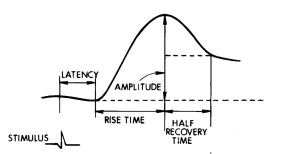
\includegraphics[width=0.7\textwidth]{images/EDAcomponents.png}
\caption{Principal EDA components}
\label{fig:EDAcomponents}
\end{figure}

\section{The experiment}
%\chapter{Experimental setup}
\label{sec:experiment}

This section summarises the relevant details of the clinical study, as
well as the main characteristics of the system used for the
acquisition of the input signals of the implemented algorithms. It
must be highlighted that the aforesaid system was not developed during
this project, but as part of the Final Degree Project of the
author \cite{Irene:PFC:2014}.


\subsection{The patients}
\label{subsec:thepatients}

Clinically, the experiment was accomplished with patients diagnosed
with migraine according to diagnostic criteria of the International
Headache Society (IHS). During the study, they took a portable
monitoring non-invasive smart system along, for a maximum of two
weeks, 24 hours a day.

Among the criteria to choose the patients, the following ones describe
the ideal profile of the volunteer:
\begin{itemize}
	\item Migraineurs aged 15 to 69 years.

	\item Migraineurs diagnosed with migraine by a headache
	specialist using ICHD-3 criteria \cite{pmid23771276}

	\item Migraineurs who have had, at least, one crisis per week
	during the last three months.

	\item Migraineurs that do not take drugs which can alter the
	variables we monitor

	\item Migraineurs with normal neurological exam

	\item Migraineurs who have signed an informed consent

	\item Migraineurs that have a minimum knowledge about using
	smartphones
\end{itemize}

Once a patient was accepted, the volunteer was asked for the
corresponding informed consent. We made an appointment with him and
the doctor in which we explained in detail the operation of the
system. Additionally, we provided the patient with a user manual of
the system in which our contacts could be found for consulting any
doubt.


\subsection{The system}
\label{subsec:thesystem}

The data acquisition was carried out with a WBSN integrated into a
broader multitier telemedicine system. The architecture implemented
involves two different sensing motes which communicate with an Android
platform via Bluetooth. The data are stored and transmitted through
the Internet to a \emph{Cloud} storage system where follow-up and
processing tasks are done.

The two used sensing motes were \emph{PLUX-Wireless Biosignals}
\cite{BIOPLUXws} and \emph{Nonin Onyx II} \cite{NONINws}. EDA, skin
temperature, ECG and EEG signals were acquired with the former and PPG
and SpO2 values were registered with the latter. The HR signal was
then calculated offline from the ECG signal by our peak-detection
algorithm. We highlight that the developed algorithms for migraine
prediction take as input a subset of four of these hemodynamic
signals: HR, EDA, skin temperature and SpO2.

The Bluetooth-enabled Android device receives the data wirelessly as
soon as each sensing mote takes a sample.  The sampling frequency for
the ECG and EEG sensors was 250 Hz, 1 Hz for the skin temperature and
EDA variables, 3 Hz for the SpO2 signal and 75 Hz for PPG.  This
introduced some synchronization issues to deal with.

The Android smartphone does not only receive and store the gathered
data, but also includes a form with questions related to every
headache. These questions include the time when the migraine phase
begins and ends, suffered symptoms and possible triggers of the
attack. The patients were asked to fill up the form as soon as a
headache has finished. Additionally, they were inquired about the
evolution of their pain intensity during the migraine crisis in order
to define a pain curve that constitutes the target signal of our
algorithms.

\section{The symptomatic pain curve}

\label{sec:paincurve}

Our purpose is to define a curve that gather the symptoms suffered by the patient during a migraine. The patients are already asked to indicate their prodromic sympotoms and the aura phase in the Android application. However, it is almost more important how the pain changes over time because it is what really incapacitates the patient during his daily life.

In order to monitor this pain evolution, the patients must register their headache intensity in real-time; \ie, indicate which is their punctual pain level at any particular moment during the migraine crisis.

Unfortunately, currently there is no way to know objectively how a patient suffers because of a headache. Instead, some tools have been approved to deal with the pain measurement. The following validated scales are among the most commonly used measures of pain intensity in clinical and research setting \cite{hawker2011measures,williamson2005pain,bashir2013comparative,ferreira2011validity}:

\begin{description}
	
	\item{\textbf{Visual Analog Scale (VAS)}\hfill \\
	It is an unidimensional measure of pain intensity which consists on a continuous scale comprised of a horizontal (HVAS) or vertical (VVAS) line, anchored by two verbal descriptors, one for each symptom extreme: ``no pain'' (score of 0) and ``pain as bad as it could be'' or ``worst imaginable pain'' (score of 100). The respondent is asked to place a line perpendicular to the VAS line at the point that represents their pain intensity. Then, the score is determined by measuring the distance on the VAS line between the ``no pain'' anchor and the mark of the patient, providing a range of scores from 0–100 where a higher score indicates greater pain intensity.
	}
	\item{\textbf{Numeric Rating Scale (NRS)}\hfill \\
	VRS is a segmented numeric version of the VAS in which the respondent selects the whole number between 0 (``no pain'') and 10 (``worst pain imaginable'') that best reflects the intensity of their pain. The NRS can be graphically or verbally delivered. Normally, when it is printed, the numbers are often enclosed in boxes.
	}
	\item{\textbf{Verbal Rating Scale (VRS)}\hfill \\
	The VRS comprises a list of adjectives used to denote increasing pain intensities. The most common words used being: ``no pain'', ``mild  pain'', ``moderate pain'',  and  ``severe/intense  pain". The respondent is asked to indicate which adjective describes better the intensity of the pain suffered. Normally, for  ease  of  recording,  each  adjectives  is assigned  numbers.
	}
	\item{\textbf{Faces Pain Scale (FPS)}\hfill \\
	It consists of six faces from left to right side in which extreme left face shows ``no pain'' while extreme right face emulates ``the worst pain imaginable''. Depending on the type of scale, faces can contain smiles, tears or just frown lines. The patients have to mark the face which best describe their intensity of pain.
	}

\end{description}

The major disadvantage of the above-mentioned scales is that the maximum level of pain is fixed, so the patients must worry about making converge the greatest intensity of their pain with the highest level of pain marked in the scale. Thus, if during the migraine crisis the ``worst pain imaginable'' level is marked and the pain increases more, the patient is not allowed to indicate this rise and the pain curve wrongly becomes saturated.

Therefore, we need a different type of scale in which the patients can always mark a higher level of intensity. We opted then in favour of monitoring relative changes of pain intensity determined by three states: more, equal or less than the last time the patient registered how the headache hurts. 
If the pain increases the patient marks a positive number, negative if decreases and 0 if it remains equal. Accordingly, the patient can disregard of when the most severe pain level is achieved and concentrate on quantifying the relative change.

In this manner, we obtain some samples of the curve of pain evolution. 
Then, in order to draw the whole curve, an adjustment process of the registered samples was carried out. 
For this purpose, in addition to the punctual points of the pain evolution, we take into account two timestamps marked during the
migraine attack: the outset and the end of the pain when detected.

The established modeling function was set as two semi-Gaussian curves, due to its simplicity and considerable fitting with the
patient's subjective response. \figref{paincurve} shows a example of this process, where the time between the two referent timestamps corresponds to the $3\sigma$ value for each semi-bell.
Also the amplitude of the final curve is normalised in order to homogenise the evolution of all the migraine crisis registered. 

\begin{figure}[!ht]
\centering
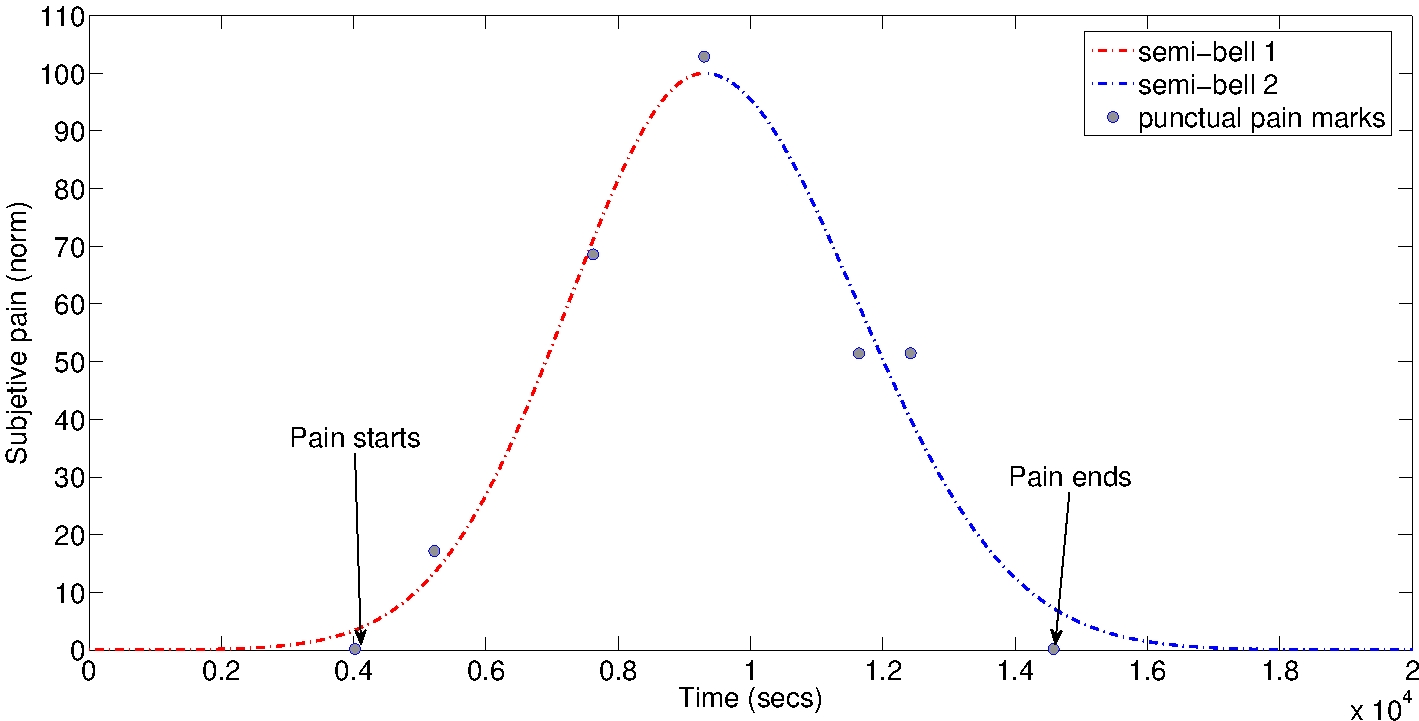
\includegraphics[width=\textwidth]{images/paincurvereal}
\caption{Modeling of subjective pain evolution curve}
\label{fig:paincurve}
\end{figure}

Nevertheless, the target signal we used in our algorithms differs slightly of the curve described.
We set the timestamp of the beginning of the aura phase as the first referent point instead of taking the beginning of pain for it. Doing this, we model other specific symptoms of the migraine disease and allow the algorithms to predict earlier the pain.

Moreover, our intention is not the modeling of the pain curve of a migraine, but only predict the its beginning. Therefore, we build a new gaussian curve setting its maximum value when the pain starts (probability of headache of 100\%). Then, the decay of the second semi-bell is determined by a sigma value of $30$ minutes. This way, we allows a fast reset of the algorithm after predicting a migraine.



% APLICACION DE ALGORITMOS
\chapter{Application of Artificial Neural Networks}
%\chapter{Application of Artificial Neural Networks}
\label{chapter:application}

After describing the biological and mathematical background of the artificial neural networks (\charef{nn}) and the adquisition process of the physiological signals we are intended to use to predict migraine (\charef{setup}), this chapter exposes the work carried out during this project.


It comprises the adaptation process of the monitored signals in order to make them suitable for being the inputs of each type of neural network. 
As far as the signals are concerned, we highlight the fact that only 4 migraine episodes of the same patient were taken into account. 
The reason of this lies on the conclusion arrived in a previous work \cite{Irene:PFC:2014}: 
the prediction goal seems to be achieve only with a per-patient model. 
Then, as the monitoring period is short, few migraines are registered from each patient.
Therefore, for the training set we used truncate version of a maximum of two migraines. Then, the test phase is carried out with the entire four migraine episodes.


It is important to emphasize that,
in order to compare and get better results,
after build and evaluate each ANN topology,
its parameters are modified and the ANN perform is reanalysed. 
The set of the adjustable params includes:
the set of signals used as network inputs,
the windowing or truncation of the time series,
the amount of neurons in the network layers, 
the number of time steps of the TDLs if they exist,
the prediction horizon  
and even the way in which the target curve is detected.
In a first instance, the greatest set of physiological variables used to predict the migraine target curve includes heart rate (HR), electrodermal activity (EDA), skin temperature (TEMP) and oxigen saturation (SpO2).

Finally, since the connection weights between neurons are randomly initialized,
we create several nets with the same ANN configuration and initialized
and trained each one independently. 
Then, we compared their performance and stored the best one.

\section{Perceptron}
%\section{Perceptron}
\label{sec:application:perceptron}
\section{Time Delay Neural Networks}

%\section{TDNN}
\label{sec:application:tdnn}
\section{Non-Linear Autorregresive model with Exogenus Input}
%\section{NARX}
\label{sec:application:NARX}
\section{Spiking Neural Networks}
%\section{Spiking Neural Networks}
\label{sec:application:snn}

\chapter{Conclusions and future work}
%\chapter{Conclusions and future work}
\label{chapter:conclusionsandfuturework}

\section{Conclusions}
\label{sec:conclusions}


\section{Future work}
\label{sec:futurework}
\chapter*{Annexes}
%\chapter*{Annexes}
\label{chapter:annexes}


\bibliographystyle{IEEEtran}
\bibliography{bib/bibtfm}

\cleardoublepage



\end{document}

